\documentclass[journal]{IEEEtran}
\usepackage{graphicx}
\usepackage{amsmath,amssymb}
\usepackage{booktabs}
\usepackage{multirow}
\usepackage[table]{xcolor}
\usepackage{tikz}
\usetikzlibrary{positioning,arrows.meta}
\usepackage[colorlinks=true,linkcolor=blue,citecolor=blue,urlcolor=blue]{hyperref}

\newcommand{\method}{TriPoseFusion~v2}
\newcommand{\methodshort}{TPF-v2}
\newcommand{\da}{Drive\&Act}
\newcommand{\best}[1]{\textbf{#1}}

\begin{document}

\title{TriPoseFusion~v2: Self-Calibrated Multi-View Fusion of Monocular 3D Keypoints\\for In-Cabin Driver Pose Estimation}

\author{Kaixu~Chen%
\thanks{K.~Chen is with XXX University, XXX, Japan (e-mail: chenkaixusan@gmail.com). \emph{(TODO: co-authors, affiliations, and funding acknowledgment.)}}%
}

\markboth{IEEE Transactions on Intelligent Transportation Systems}%
{Chen \MakeLowercase{\textit{et al.}}: TriPoseFusion v2}

\maketitle

\begin{abstract}
Driver monitoring systems need stable 3D body pose under occlusion, constrained camera placement, and rapidly changing illumination. Off-the-shelf monocular 3D pose estimators can be deployed per camera, but their outputs live in inconsistent coordinate frames and exhibit view-dependent errors, and obtaining metric 3D ground truth inside a vehicle cabin is impractical. This paper presents a complete, self-calibrated pipeline for fusing synchronized tri-view monocular 3D keypoints. First, we show that a multi-view triangulation reference built with nominal camera extrinsics suffers per-session scale errors of up to $6\times$, and we introduce a per-sequence self-calibration procedure---robust bundle adjustment of the camera extrinsics from the 2D keypoint observations themselves, with the metric scale gauge anchored to the monocular estimator's body-size prior---that reduces the reference reprojection error from 9.6 to 3.3\,px and its cross-session shoulder-width spread from $0.46$--$2.10$\,m to $0.368\pm0.015$\,m without any calibration target or manual 3D annotation. Second, we present \method{}, a lightweight fusion network (28K parameters, $<$0.6\,ms per frame on one CPU thread) that combines masked set attention over any subset of views, corruption-aware gating trained with view-corruption augmentation, a residual refinement head supervised by the self-calibrated triangulation reference, and a per-joint uncertainty output. On 88 subject-environment sequences under four illumination conditions and subject-disjoint 5-fold evaluation, \method{} reduces MPJPE by 11.8\% and hand error by 11\% over the strongest training-free fusion baseline; when one camera fails, its accuracy degrades by less than 7\% while assigning the corrupted view a weight of 0.01--0.03, matching an oracle that knows which view is corrupted. The predicted uncertainty correlates with the actual error (Spearman $\rho=0.74$). On the public \da{} benchmark, the training-free canonicalized fusion transfers zero-shot at 23.1\,mm PA-MPJPE, and re-running the label-free adaptation recipe on the new rig improves it to 19.9\,mm. We further contribute two cautionary analyses of broad relevance: a proof that consensus-teacher self-supervision collapses multi-view gating to uniform averaging, and a demonstration of how reference-scale errors manufacture illusory learning gains.
\end{abstract}

\begin{IEEEkeywords}
Driver monitoring, 3D human pose estimation, multi-view fusion, self-calibration, intelligent vehicles.
\end{IEEEkeywords}

\IEEEpeerreviewmaketitle

\section{Introduction}
\IEEEPARstart{D}{river} monitoring and in-cabin behavior understanding rely on stable 3D representations of the driver's body. Fine-grained pose supports attention estimation, hand-state analysis, gesture understanding, and safety intervention \cite{abouelnaga2017real,zhang2018driver,gorelik2026multiview}. The in-cabin setting is heavily constrained: the driver is seated, cameras are mounted at fixed but vehicle-specific positions, and safety-critical motion is concentrated in a small upper-body workspace. The same constraints create persistent visual challenges---steering-wheel and self-occlusion, limited viewpoints, and abrupt illumination changes between day and night driving.

Monocular 3D pose estimators \cite{toshev2014deeppose,martinez2017simple,mehta2017vnect,kanazawa2018end} are attractive here because they run independently per camera and need no reconstruction infrastructure. Their predictions, however, are depth-ambiguous and view-dependent: each camera returns keypoints in its own root-relative frame, with its own bias pattern, missing joints, and jitter. A multi-camera rig observes complementary evidence \cite{iskakov2019learnable,qiu2019cross,tu2020voxelpose}, but exploiting it at the \emph{keypoint level}---the natural interface when the per-view estimator is an off-the-shelf component---raises three coupled problems that this paper addresses end to end.

\emph{(1) The reference problem.} Learning and evaluating multi-view fusion requires a 3D reference, yet motion capture is impractical in a cabin and even checkerboard calibration is difficult to repeat every time a rig is serviced or re-mounted. The common workaround, triangulating 2D keypoints with nominal (assumed) extrinsics, is dangerous in a way that is easy to miss: we show that on our 22-subject dataset the nominal-extrinsics reference has a median body-scale error of $2.4\times$ that varies by recording session from $1.2\times$ to $6\times$ (Sec.~\ref{sec:reference}), because the rig geometry differed across sessions. All ``metric'' errors computed against such a reference are dominated by reference-scale error, not pose error.

\emph{(2) The fusion problem.} Given well-aligned views, how much can a learned fusion module improve over simple averaging, and where? We answer this with a strictly controlled protocol (identical inputs, references, masks, and metrics for every method) and find a nuanced picture: learned \emph{view weighting} alone offers no accuracy gain---and we prove why its self-supervised variant cannot (Sec.~\ref{sec:collapse})---whereas a small \emph{residual refinement} head supervised by the self-calibrated reference gives consistent gains, concentrated on the hardest joints (hands).

\emph{(3) The robustness and transfer problem.} A deployed system must tolerate a failed or corrupted camera, and a method developed on one rig must be transferable to another. We show that corruption-aware training makes gating match an oracle that knows which view failed, and that residual refinement is inherently rig-specific---it degrades under zero-shot transfer but is restored, without any manual labels, by re-running the same self-calibrated adaptation recipe on the target rig.

This paper is a substantially revised and corrected successor of an earlier conference submission describing TriPoseFusion. In re-auditing that system we found that its headline improvements were artifacts of evaluation defects (an inverted Procrustes rotation, a degenerate canonicalization fallback) and of the reference-scale error above; we document these findings here as analyses (Secs.~\ref{sec:collapse} and \ref{sec:scaleartifact}) because they concern failure modes that can affect any work that trains or evaluates against pseudo ground truth.

Our contributions are:
\begin{itemize}
\item \textbf{A self-calibrated triangulation reference for in-cabin rigs.} Per-sequence robust bundle adjustment of camera extrinsics from the 2D keypoint observations themselves, with the scale gauge anchored to the monocular estimator's body-size prior. No calibration target, no manual 3D annotation. Reference reprojection error drops from 9.6 to 3.3\,px, the front-view utilization rises from 8\% to 45\%, and the cross-session shoulder-width spread collapses from std 0.37\,m to 0.015\,m (Table~\ref{tab:gtquality}).
\item \textbf{\method{}, a lightweight, deployment-oriented fusion network.} Masked set attention over the available views (any subset of 1--3 cameras), corruption-aware gating trained with view-corruption augmentation, residual refinement supervised by the self-calibrated reference, and a per-joint Laplace uncertainty output. 27.9K parameters; $<$0.6\,ms per frame on a single CPU thread.
\item \textbf{A controlled benchmark and honest accounting of where learning helps.} Under subject-disjoint 5-fold evaluation, \method{} improves MPJPE by 11.8\%, hand error by 11\%, and PCK@0.10 by $+4.1$ points over the strongest training-free fusion; view weighting alone contributes nothing; under a corrupted camera, accuracy is maintained within 7\% (vs.\ 19\% degradation for averaging), matching an oracle exclusion.
\item \textbf{Cross-rig validation on \da{}} \cite{martin2019drive}: training-free canonicalized fusion transfers zero-shot (23.1\,mm PA-MPJPE, on par with fully supervised methods trained on that benchmark), and the label-free adaptation recipe reduces it to 19.9\,mm (leave-one-subject-out).
\item \textbf{Two cautionary analyses}: a proof that consensus-teacher self-supervision makes uniform view weighting the loss-optimal solution (explaining ``gate collapse'' observations), and a quantified case study of how reference-scale errors manufacture illusory learning gains that do not transfer.
\end{itemize}

\section{Related Work}
\label{sec:related}

\subsection{Monocular and Video 3D Pose Estimation}
Monocular 3D pose is recovered by direct regression, 2D-to-3D lifting, or body-model fitting \cite{toshev2014deeppose,martinez2017simple,zhou2017towards,mehta2017vnect,kanazawa2018end}, with temporal models reducing jitter \cite{pavllo20193d,kocabas2020vibe}. In-cabin conditions---steering-wheel occlusion, truncation, extreme illumination---remain difficult for single views. We treat monocular outputs as noisy observations and study their fusion, rather than proposing another estimator.

\subsection{Multi-View Pose Estimation and Keypoint-Level Fusion}
Multi-view methods triangulate 2D detections with calibrated cameras \cite{hartley1997triangulation,iskakov2019learnable}, exchange image features across views \cite{qiu2019cross,he2020epipolar}, or aggregate volumetrically \cite{tu2020voxelpose,bultmann2021real,nogueira2024markerless}. These assume image access and calibrated cameras at inference. Our interface is deliberately narrower: the fusion stage receives only per-view 3D keypoints from an off-the-shelf estimator, needs no calibration at deployment (calibration is used only to build the training reference), and runs in microseconds. This keypoint-level setting exposes problems---inconsistent per-view frames, missing joints, time-varying reliability---that image-level methods do not face, and that simple averaging does not solve under camera failure.

\subsection{Self-Supervision, Pseudo Labels, and Their Failure Modes}
Without mocap, prior work uses reprojection consistency, multi-view agreement, bone priors, temporal smoothness, or triangulated pseudo labels \cite{rhodin2018learning,kocabas2019self,iskakov2019learnable,wandt2021canonpose,fan2023humanm3}. We contribute two failure-mode analyses to this line: consensus-teacher objectives provably drive adaptive view weighting to uniform averaging (Sec.~\ref{sec:collapse}), and scale errors in a pseudo reference can be silently ``learned'' by a refinement network, inflating apparent gains that vanish under transfer (Sec.~\ref{sec:scaleartifact}). Our reference construction is closest in spirit to self- or auto-calibration from human keypoints; unlike prior setups we calibrate \emph{per recording session} and anchor the metric scale to the monocular estimator's body prior, which we validate against physically plausible anatomy.

\subsection{Driver Monitoring Datasets}
\da{} \cite{martin2019drive} provides multi-view in-cabin recordings with OpenPose-triangulated 3D references and is our cross-rig testbed. Our own dataset complements it with a three-camera RGB rig, 22 subjects, four illumination conditions, and a 52-keypoint protocol that includes both hands.

\section{Self-Calibrated Triangulation Reference}
\label{sec:reference}

\subsection{Setup and the Nominal-Extrinsics Problem}
Our rig has three cameras (front, left, right) observing the seated driver. Each view runs the same off-the-shelf monocular estimator (SAM3D-Body), which outputs 70 2D/3D keypoints per frame; a 52-keypoint subset (head, shoulders/neck, and both hands) is used throughout. The reference is built by triangulating the synchronized 2D keypoints \cite{hartley1997triangulation}: for each joint, every view subset of size $\geq 2$ is triangulated by DLT, the subset with the lowest mean reprojection error is kept (ties broken toward more views), points behind any used camera or above a 40\,px error threshold are rejected, and per-point quality statistics (reprojection error, leave-one-view-out displacement, condition number) are stored.

Intrinsics were estimated once per camera. Extrinsics, however, were originally \emph{constructed} from a nominal layout (look-at poses from measured distances and a 0.70\,m left--right baseline). Auditing the resulting reference against anatomy exposed a serious defect: the median triangulated shoulder width across the 88 sequences was 0.84\,m---more than twice a plausible human value---and ranged from 0.46\,m to 2.10\,m depending on the \emph{subject}, i.e., on the recording session (Table~\ref{tab:gtquality}, first row). The estimator's own metric body prior was, by contrast, extremely stable (median shoulder width 0.371\,m, spread $<$0.06\,m across all views and sequences). The conclusion is that the rig was re-positioned between sessions while a single nominal geometry was assumed; the induced errors are mostly \emph{scale-like}, so they poison every metric error computed against the reference while remaining invisible to reprojection-based quality checks.

\subsection{Per-Sequence Robust Extrinsic Refinement}
We therefore refine extrinsics \emph{per sequence}, using the 2D keypoint observations themselves as correspondences. The left camera is fixed as the gauge; the 6-DoF poses of the front and right cameras are optimized by minimizing the Huber-robustified reprojection error of DLT-triangulated points over roughly 40 frames sampled evenly from the sequence, in two rounds with outlier rejection in between. A soft prior keeps the solution near the nominal layout. Across 88 sequences the refinement rotates the nominal camera orientations by a median of 21$^\circ$ (front) and 31$^\circ$ (right)---up to 53$^\circ$---confirming that the nominal layout was substantially wrong; held-out frames show the mean reprojection error dropping from 9.6 to 3.4\,px and the front camera's participation in accepted triangulations rising from 8\% to 45\%.

\subsection{Anchoring the Scale Gauge}
Rotation refinement alone cannot fix scale: with unknown extrinsics, the global scale of the reconstruction is a gauge freedom (scaling the scene about the fixed camera leaves all reprojections unchanged), and pinning it with the nominal 0.70\,m baseline is exactly what failed---the true baseline differed per session (we recover 0.25--1.07\,m, median 0.80\,m). We instead anchor the gauge \emph{anatomically}: for each sequence, the scene is rescaled about the fixed camera so that the median triangulated shoulder width equals the monocular estimator's median metric shoulder width for that sequence. This choice (i) costs nothing in reprojection error, (ii) makes the reference's metric scale consistent with the input streams being fused, and (iii) is validated by convergence: the resulting shoulder widths are $0.368\pm0.015$\,m across all 88 sequences, in agreement with both the estimator prior (0.371\,m) and human anatomy.

\begin{table}[t]
\centering
\caption{Reference quality across the three extrinsics variants (88 sequences, $\sim$0.7M frames per camera). ``Shoulder width'' is the per-sequence median of the triangulated left--right shoulder distance; a physically plausible reference must concentrate near 0.37\,m.}
\label{tab:gtquality}
\scriptsize
\setlength{\tabcolsep}{3pt}
\begin{tabular}{lccc}
\toprule
Extrinsics & Valid joints & Mean reproj.\ (px) & Shoulder width (m) \\
\midrule
Nominal layout & 35.8\% & 9.60 & 0.839 [0.46, 2.10], $\sigma{=}0.369$ \\
Global refinement & 37.8\% & 5.18 & 0.410 [0.28, 3.85], $\sigma{=}0.422$ \\
\textbf{Per-seq.\ + anchor} & 37.7\% & \best{3.31} & \best{0.368 [0.325, 0.389], $\sigma{=}0.015$} \\
\bottomrule
\end{tabular}
\end{table}

Table~\ref{tab:gtquality} summarizes the three stages. A single globally refined extrinsics set (middle row) already halves the reprojection error but cannot fix sessions whose geometry differs from the calibration subset; only the per-sequence procedure with anatomical anchoring yields a reference that is simultaneously low-error and scale-consistent. All experiments below use this reference; Sec.~\ref{sec:scaleartifact} quantifies what happens when the first-row reference is used instead.

\section{TriPoseFusion v2}
\label{sec:method}
% TODO(figure): add a v2 pipeline overview figure (canonicalization -> masked set attention
% -> gate/residual/uncertainty heads); figures/flow_chart.png shows the outdated v1 design.
% TODO(figure): add a qualitative comparison figure rendered against the self-calibrated
% reference (the old fig_qualitative_pose.pdf was rendered against the mis-scaled reference).

\subsection{Problem Setting and Canonicalization}
At inference, \method{} receives synchronized monocular 3D keypoint streams $P_v \in \mathbb{R}^{T\times J\times 3}$ from the available views $v \in \mathcal{V}$, $1 \le |\mathcal{V}| \le 3$, $J{=}52$, and outputs a fused sequence plus a per-joint uncertainty. No camera calibration and no images are needed at inference; the calibrated reference of Sec.~\ref{sec:reference} is used only as the training signal.

Each view is first canonicalized into a body-centered frame: the neck is the origin, the $x$ axis is the normalized right-to-left shoulder direction, the downward axis is the shoulder midpoint minus the neck, and the frame is orthonormalized by cross products. Two robustness rules matter in practice: if a frame's shoulder estimate is degenerate (coincident or anatomically implausible), the shoulder axis of the temporally nearest valid frame is reused (never a zero vector, which would collapse the rotation); and if the shoulder and torso axes become near-parallel, a fixed reference axis restores full rank. Canonicalization is what makes per-view streams commensurable: on our data it reduces the cross-view disagreement of raw monocular outputs from the 2\,m scale (root-relative camera frames) to the 0.15\,m scale.

\subsection{Masked Set Attention over Views}
For each joint $j$ and frame $t$, the $|\mathcal{V}|$ canonicalized observations form a token set. Each token embeds its 3D coordinates, its distance to the finite-view mean (a cross-view-consistency cue), a finite-validity flag, and learned view and joint embeddings. Two transformer encoder layers operate \emph{across the view set} with key masking of missing views; because attention over a set is permutation-equivariant \cite{zaheer2017deep}, the same network handles any subset of cameras, and a view that drops out at runtime is excluded exactly like a view that was never present.

A linear head maps each attended token to a gate logit; a masked softmax yields per-joint, per-frame view weights $\alpha_{t,j,v}$ and the gated fusion $\hat{p}_{t,j} = \sum_v \alpha_{t,j,v} \bar{P}^{t,j}_v$. The attention-pooled feature is then processed by one transformer layer across the $J$ joints (skeleton context, e.g., wrist evidence informing finger corrections) and a depthwise temporal convolution (kernel 5), and two zero-initialized heads output a residual correction $\Delta_{t,j} \in \mathbb{R}^3$ and a per-joint Laplace log-scale $s_{t,j}$:
\begin{equation}
p^{\mathrm{out}}_{t,j} = \hat{p}_{t,j} + \Delta_{t,j}, \qquad
\sigma_{t,j} = \exp(s_{t,j}).
\end{equation}

\subsection{Training: Triangulation Supervision, Corruption Augmentation, Uncertainty}
\label{sec:training}
The only loss is a masked Laplace negative log-likelihood against the self-calibrated reference $g_{t,j}$ over its valid joints:
\begin{equation}
\mathcal{L} = \frac{1}{|\Omega|}\sum_{(t,j)\in\Omega} \Big( \|p^{\mathrm{out}}_{t,j}-g_{t,j}\|_1 \, e^{-s_{t,j}} + 3\, s_{t,j} \Big),
\label{eq:nll}
\end{equation}
which trains the residual head and calibrates the uncertainty jointly \cite{kendall2017uncertainties}. During training, with probability 0.5 per sample one random view is corrupted---dropped (masked), zeroed, or perturbed with $\sigma{=}0.1$\,m Gaussian noise. This \emph{corruption augmentation} is what teaches the gate to detect and down-weight unreliable views; without it, we find the gate has no incentive to encode reliability (Sec.~\ref{sec:robustness}).

Three deliberate simplicity choices follow from our analyses. (i) \emph{No consensus self-supervision}: the v1 objective used the multi-view median as a teacher, for which uniform weighting is provably optimal (Sec.~\ref{sec:collapse}). (ii) \emph{No contrastive view alignment}: InfoNCE between view features actively erases the inter-view differences the gate must read. (iii) \emph{Small capacity}: the deployed model uses $d{=}32$ (27.9K parameters); we show that $30\times$ larger variants do not help and the v1-scale backbone (0.87M) overfits (Sec.~\ref{sec:ablation}).

\subsection{Why Consensus Self-Supervision Collapses Gating}
\label{sec:collapse}
The v1 system trained the fused pose against the per-frame coordinate-wise \emph{median} of its own canonicalized inputs, plus self-referential consistency terms. Observe that the fusion output is a $\alpha$-weighted convex combination of the inputs, and the objective is minimized over $\alpha$ by whichever combination best approximates a robust central tendency of those same inputs; in the symmetric-noise regime this is the uniform average, and no input pattern carries information that could break the symmetry. The prediction is specific: gates should converge to exactly $1/V$ regardless of architecture or capacity. Empirically, every retrained configuration of the v1 system (with or without cross-view attention, with different regularization weights, and with a leave-one-view-out teacher variant) converged to gates of $0.333/0.333/0.333$ and an output indistinguishable from mean fusion---under our unified protocol, the v1 model scores $0.1857$\,m MPJPE vs.\ $0.1858$\,m for plain mean fusion. The same collapse reproduced zero-shot on \da{}. Adaptive multi-view weighting requires an information source \emph{external} to the views being weighted: here, the triangulation reference and the corruption augmentation.

\subsection{How Reference-Scale Errors Manufacture Illusory Gains}
\label{sec:scaleartifact}
Against the nominal-extrinsics reference of Table~\ref{tab:gtquality} (first row), a 1.9K-parameter fusion model with a temporal head appeared to beat mean fusion by 12.5\% MPJPE. The gain was an artifact: the reference is on average $2.4\times$ too large, so the network's temporal convolution learned a global inflation of the output (measured output scale $2.1\times$ the input scale), which \emph{reduces} error against the mis-scaled reference while corrupting the pose. The tell-tale signatures were (i) the gain disappeared when the temporal head was removed, (ii) PCK and rigid-alignment errors moved opposite to MPJPE, and (iii) zero-shot transfer to \da{} \emph{degraded} from 23.1 to 28--37\,mm PA-MPJPE. After scale anchoring, the same model's gain over mean fusion is $0.4\%$, i.e., zero. We report this case study because pseudo-ground-truth supervision is widespread; a scale-consistent reference (or at minimum a scale-invariant metric) is a prerequisite for claiming learned improvements.

\section{Experiments}
\label{sec:experiments}

\subsection{Dataset, Protocol, and Baselines}
\begin{figure}[t]
\centering
\begin{minipage}[t]{0.235\linewidth}
\centering
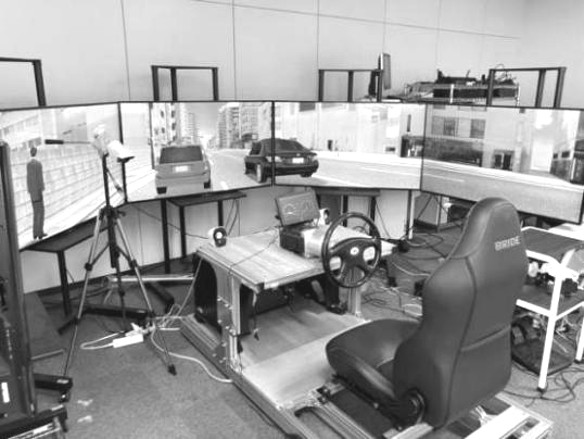
\includegraphics[width=\linewidth]{figures/dataset/driving_simulator.jpg}\\[-1mm]
{\scriptsize (a) Simulator}
\end{minipage}
\hfill
\begin{minipage}[t]{0.235\linewidth}
\centering
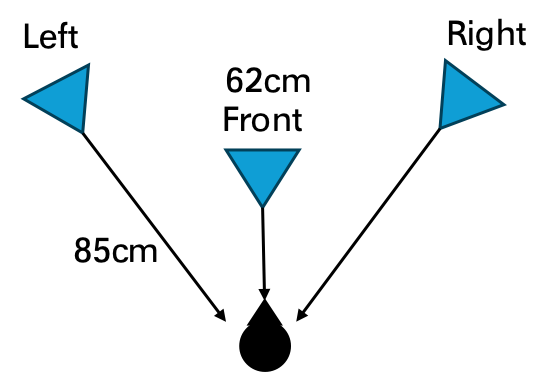
\includegraphics[width=\linewidth]{figures/dataset/camera_config.png}\\[-1mm]
{\scriptsize (b) Cameras}
\end{minipage}
\hfill
\begin{minipage}[t]{0.235\linewidth}
\centering
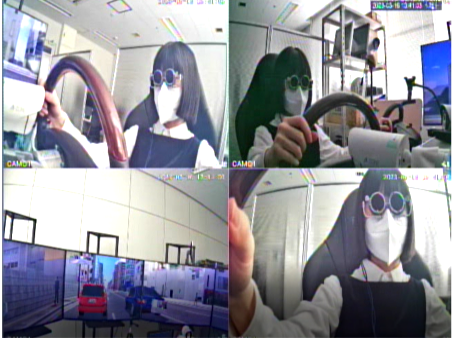
\includegraphics[width=\linewidth]{figures/dataset/day.png}\\[-1mm]
{\scriptsize (c) Daytime}
\end{minipage}
\hfill
\begin{minipage}[t]{0.235\linewidth}
\centering
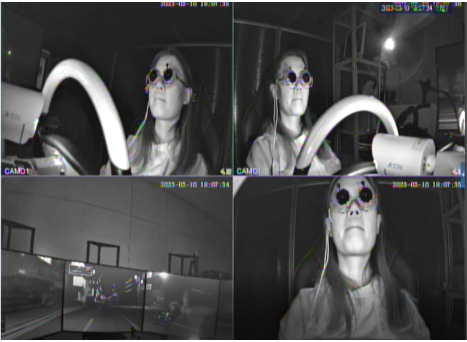
\includegraphics[width=\linewidth]{figures/dataset/night.png}\\[-1mm]
{\scriptsize (d) Nighttime}
\end{minipage}
\caption{In-cabin acquisition setting: driving simulator, fixed tri-view camera rig, and representative daytime/nighttime frames illustrating illumination change, steering-wheel occlusion, and view-dependent visibility. Note that camera placement varied across recording sessions, which motivates the per-sequence self-calibration of Sec.~\ref{sec:reference}.}
\label{fig:dataset}
\end{figure}

\textbf{In-cabin dataset} (Fig.~\ref{fig:dataset}). 22 subjects, four illumination settings (day/night $\times$ high/low), one sequence per subject and setting: 88 sequences, $\sim$0.7M frames per camera. Each camera stream is processed by SAM3D-Body; the model input is the 52-keypoint subset covering the head (5), shoulders/neck (5), and both hands (42). The evaluation reference is the self-calibrated triangulation of Sec.~\ref{sec:reference}; metrics are computed on its valid joints only ($\sim$17M joint observations).

\textbf{Protocol.} Subject-disjoint GroupKFold with 5 folds; every learned model is trained for a fixed number of steps with a fixed seed and evaluated at the final step (no model selection on the evaluation fold). All methods---training-free and learned---consume the identical cached canonicalized inputs, the identical reference, the identical validity masks, and the identical metric code. We report MPJPE, PA-MPJPE (Procrustes with the correct least-squares similarity solution \cite{umeyama1991least}), and PCK@0.10\,m, as mean $\pm$ std over folds; joint-group breakdowns (head / shoulders--neck / body / hands); and, for robustness, errors under single-view corruption.

\textbf{Baselines.} Per-view single baselines; the per-sequence \emph{oracle} best single view; training-free canonicalized mean and median fusion; a gating-only learned model (1.9K parameters, no residual head); and the v1 backbone (view encoder, cross-view attention, gate, dilated TCN) retrained with our supervision at two capacities.

\begin{table}[t]
\centering
\caption{Main comparison on the in-cabin dataset (5-fold, subject-disjoint; m). All rows share identical inputs, reference, masks, and metric code. $\Delta$ is the paired per-fold MPJPE change vs.\ mean fusion.}
\label{tab:main}
\scriptsize
\setlength{\tabcolsep}{2.2pt}
\begin{tabular}{lccccc}
\toprule
Method & Params & MPJPE $\downarrow$ & PA-MPJPE $\downarrow$ & PCK@0.10 $\uparrow$ & $\Delta$ \\
\midrule
Front only & -- & $0.172{\pm}.025$ & $0.059{\pm}.011$ & $0.459$ & $+16\%$ \\
Left only & -- & $0.161{\pm}.029$ & $0.046{\pm}.011$ & $0.473$ & $+8\%$ \\
Right only & -- & $0.152{\pm}.025$ & $0.045{\pm}.010$ & $0.477$ & $+3\%$ \\
Median fusion & -- & $0.152{\pm}.024$ & $0.046{\pm}.010$ & $0.485$ & $+2\%$ \\
Mean fusion & -- & $0.149{\pm}.026$ & $0.044{\pm}.009$ & $0.497$ & -- \\
Best single (oracle) & -- & $0.145{\pm}.022$ & $0.046{\pm}.012$ & $0.488$ & $-2.6\%$ \\
\midrule
Gating-only + aug. & 1.9K & $0.149{\pm}.026$ & $0.044{\pm}.009$ & $0.503$ & $+0.4\%$ \\
v1 backbone retrained & 261K & $0.136{\pm}.032$ & $0.042{\pm}.009$ & $0.535$ & $-9.0\%$ \\
Residual-only + aug. & 8.0K & \best{$0.128{\pm}.031$} & \best{$0.040{\pm}.010$} & \best{0.548} & \best{$-14.3\%$} \\
\textbf{\method{} (full)} & 27.9K & $0.132{\pm}.031$ & $0.042{\pm}.009$ & $0.538$ & $-11.8\%$ \\
\bottomrule
\end{tabular}
\end{table}

\subsection{Main Results}
Table~\ref{tab:main} gives the central accuracy picture. Three observations. \emph{First}, canonicalized mean fusion is a strong baseline: it beats every individual camera and is within 3\% of the per-sequence oracle camera; the value of having three views on this rig comes mostly from robustness, not clean accuracy. \emph{Second}, learned view weighting adds nothing (gating-only: $+0.4\%$; learned weights $\approx$ uniform)---as predicted by Sec.~\ref{sec:collapse}, and now confirmed even with reference supervision, because the oracle view-selection headroom is only 2.6\%. \emph{Third}, residual refinement is the one real accuracy lever: the 8K residual-only model improves MPJPE by 14.3\% and the full model by 11.8\%, both surpassing the oracle single view. Per joint group (Table~\ref{tab:groups}), the improvement concentrates where monitoring needs it most: hands ($0.234\to0.208$, $-11\%$) and head ($-10\%$), with shoulder/neck slightly degraded (these near-origin joints define the canonical frame and are already at 2\,cm).

\begin{table}[t]
\centering
\caption{MPJPE by joint group (5-fold mean, m).}
\label{tab:groups}
\scriptsize
\setlength{\tabcolsep}{4pt}
\begin{tabular}{lcccc}
\toprule
Method & Head & Shoulders/neck & Body & Hands \\
\midrule
Mean fusion & 0.081 & \best{0.022} & 0.052 & 0.234 \\
Best single (oracle) & 0.080 & 0.023 & 0.051 & 0.234 \\
\method{} (full) & \best{0.073} & 0.025 & \best{0.049} & \best{0.208} \\
\bottomrule
\end{tabular}
\end{table}

\subsection{Robustness to Camera Corruption}
\label{sec:robustness}
Table~\ref{tab:stress} evaluates the failure mode that motivates multi-camera rigs: one view becomes unusable at runtime. Three corruption types are applied to each view in turn on the evaluation folds: \emph{drop} (the view is absent), \emph{zero} (the stream returns a constant pose---an undetected failure), and \emph{noise} ($\sigma{=}0.1$\,m). Mean fusion degrades by 19\% under zeroing because it ingests the corrupted stream at fixed weight $1/3$. \method{} assigns the zeroed view a weight of 0.01--0.03 and keeps its error within 7\% of the clean value---\emph{better} than the oracle that excludes the corrupted view but loses its residual corrections. The ablation row shows corruption augmentation is the necessary ingredient: without it the model up-weights corrupted views (weight 0.31) and degrades below the averaging baseline. Gaussian noise is harder to detect than zeroing (weights 0.09--0.38), identifying a limitation.

\begin{table}[t]
\centering
\caption{Single-view corruption at test time (5-fold mean over the three corrupted views; MPJPE, m). ``$w$'' is the mean gate weight assigned to the corrupted view (uniform $=0.33$). Oracle removes the corrupted view by fiat.}
\label{tab:stress}
\scriptsize
\setlength{\tabcolsep}{3.2pt}
\begin{tabular}{lcccc}
\toprule
Method & Clean & Drop & Zero ($w$) & Noise ($w$) \\
\midrule
Mean fusion & 0.149 & 0.152 & 0.176 (0.33) & 0.167 (0.33) \\
Oracle excl.\ view & -- & 0.152 & 0.152 (0) & 0.152 (0) \\
\method{} w/o aug. & 0.132 & -- & 0.178 (0.31) & -- \\
\textbf{\method{} (full)} & \best{0.132} & \best{0.136} & \best{0.137 (0.02)} & \best{0.137 (0.22)} \\
\bottomrule
\end{tabular}
\end{table}

\subsection{Cross-Rig Evaluation on \da{}}
\label{sec:driveandact}
\da{} \cite{martin2019drive} provides an independent rig (NIR cameras: inner mirror, both A-pillars), an independent reference (multi-view OpenPose triangulation), and different subjects. We evaluate on the official split-0 test subjects (vp5, vp11, vp13; six runs; dense 30\,fps clips), on the joints shared between our 52-keypoint space and BODY-25.

\textbf{Zero-shot.} Running the same monocular estimator per view and our training-free canonicalize-and-average fusion yields 23.1\,mm pooled PA-MPJPE---in the range of fully supervised methods trained on \da{} (22.6--30.4\,mm as cited in prior work), and 4--27\% better than the best single view. The gating-only model transfers unchanged (23.1\,mm). Models with residual heads, however, degrade (28.6\,mm full model; 36\,mm residual-only): the corrections they learned encode \emph{this-rig-and-estimator-specific} systematic error, and the learned view priors even invert (front is the least trusted view on our rig, the most trusted on \da{}).

\textbf{Label-free in-domain adaptation.} The correct deployment recipe is therefore to re-run the adaptation on the target rig: build the triangulation reference from the rig's own observations (here \da{}'s own reference) and retrain the tiny fusion network---minutes of CPU time, no manual labels. Under leave-one-subject-out (Table~\ref{tab:da}), the residual-only model reaches $18.6$\,mm PA-MPJPE ($-23\%$ vs.\ training-free fusion), the full model $19.9$\,mm ($-18\%$), and wrist error drops by 27\%; under a zeroed camera the adapted full model degrades to 24\,mm while averaging degrades to 84\,mm.

\begin{table}[t]
\centering
\caption{\da{}, leave-one-subject-out adaptation (3 folds; shared upper-body joints; m).}
\label{tab:da}
\scriptsize
\setlength{\tabcolsep}{3.2pt}
\begin{tabular}{lccc}
\toprule
Method & MPJPE $\downarrow$ & PA-MPJPE $\downarrow$ & Wrists $\downarrow$ \\
\midrule
Best single view (right) & $0.0343{\pm}.003$ & $0.0261{\pm}.003$ & 0.071 \\
Median fusion & $0.0266{\pm}.002$ & $0.0251{\pm}.002$ & 0.041 \\
Mean fusion & $0.0247{\pm}.002$ & $0.0243{\pm}.002$ & 0.035 \\
Gating-only + aug. & $0.0235{\pm}.002$ & $0.0228{\pm}.002$ & 0.033 \\
Residual-only & \best{$0.0203{\pm}.002$} & \best{$0.0186{\pm}.002$} & \best{0.026} \\
\textbf{\method{} (full)} & $0.0217{\pm}.002$ & $0.0199{\pm}.002$ & 0.030 \\
\bottomrule
\end{tabular}
\end{table}

\subsection{Uncertainty Calibration}
The Laplace scale output orders errors well: Spearman correlation between predicted scale and realized per-joint error is $0.74$ on the in-cabin folds and $0.51$ on adapted \da{}. Selecting the most-confident decile of joints yields 1.6\,cm mean error versus 27\,cm for the least-confident decile (14.8\,cm overall)---directly usable by downstream monitoring logic to suppress unreliable joints. This capability has no training-free counterpart.

\subsection{Ablations and Capacity}
\label{sec:ablation}
Table~\ref{tab:ablation} isolates the contributions. Removing corruption augmentation leaves clean accuracy unchanged but destroys robustness (Sec.~\ref{sec:robustness}). Removing the skeleton-attention layer or the temporal convolution changes accuracy by $\leq 0.3\%$---consistent with the residual head being the active ingredient---so deployments free to drop them can use the 19.4K variant. Capacity beyond 8--28K parameters does not help: a 92K residual variant is flat, and the retrained v1 backbone at its original capacity (870K) is the \emph{worst} learned model ($-4.2\%$, per-fold range $-21\%$ to $+26\%$), overfitting 68 training sequences. On efficiency: the full model runs in $<$0.6\,ms per frame on one CPU thread (residual-only: 0.08\,ms), and one training fold takes $\sim$8 CPU-minutes---adaptation to a new vehicle is computationally trivial.

\begin{table}[t]
\centering
\caption{Ablations (5-fold; in-cabin dataset; m).}
\label{tab:ablation}
\scriptsize
\setlength{\tabcolsep}{3.5pt}
\begin{tabular}{lcccc}
\toprule
Variant & Params & MPJPE & PA-MPJPE & Zero-corr.\ MPJPE \\
\midrule
\method{} (full) & 27.9K & 0.1320 & 0.0423 & \best{0.137} \\
\;-- corruption aug. & 27.9K & 0.1324 & 0.0430 & 0.178 \\
\;-- skeleton attention & 19.4K & 0.1323 & \best{0.0408} & -- \\
\;-- temporal conv. & 27.7K & 0.1323 & 0.0424 & -- \\
Residual-only + aug. & 8.0K & \best{0.1284} & 0.0402 & \best{0.132} \\
Residual (large) & 92K & 0.1311 & 0.0435 & -- \\
v1 backbone (h64) + aug. & 261K & 0.1359 & 0.0416 & 0.138 \\
v1 backbone (h128) & 870K & 0.1423 & 0.0437 & -- \\
\bottomrule
\end{tabular}
\end{table}

\section{Discussion and Limitations}
Our results reframe what a learned in-cabin fusion module should claim. On a healthy three-camera rig, training-free canonicalized averaging is nearly optimal for clean accuracy, and the honest value of learning lies elsewhere: robustness to camera failure (at oracle level, for free), rig-specific residual correction (worth 12--23\% where it is retrained on the target rig's own automatic reference), and calibrated per-joint confidence. Limitations remain. The reference is triangulation of the same 2D detections used by the fused streams---an independent sensor would strengthen absolute claims, and \da{}'s independent reference partially fills this role. Hands still dominate the error budget (0.21\,m vs.\ 0.05\,m for the body) and are at times invisible to all three cameras. Gaussian corruption is only partially detected by the gate. Finally, the scale anchor inherits any global bias of the monocular estimator's body prior; PA-MPJPE is unaffected, but absolute MPJPE shifts with that prior.

\section{Conclusion}
We presented a self-calibrated pipeline for multi-view driver pose estimation at the keypoint level: a per-sequence extrinsic refinement with anatomically anchored scale that turns nominal-extrinsics triangulation into a physically consistent reference (3.3\,px, $0.368\pm0.015$\,m shoulder width), and \method{}, a 28K-parameter set-attention fusion network with corruption-aware gating, reference-supervised residual refinement, and calibrated uncertainty. The system improves accuracy by 11.8\% over strong training-free fusion, tolerates a failed camera at oracle level, transfers across rigs via minutes of label-free adaptation (\da{} PA-MPJPE 19.9\,mm), and runs in microseconds per frame. The accompanying analyses---consensus self-supervision provably collapses view gating, and reference-scale errors manufacture illusory gains---are cautionary results we believe generalize well beyond driver monitoring.

\bibliographystyle{IEEEtran}
\bibliography{refs,extra}

\end{document}
